% AA-64
\chapter[Podalgebry Cartana i rozkład Fittinga]{Podalgebry Cartana, rozkład Fittinga i elementy regularne}
\label{aa:ch:cartan-fitting}

W AA-59 wykazaliśmy, że maksymalna podalgebra toralna algebry półprostej jest podalgebrą Cartana, a w AA-63 udowodniliśmy sprzężoność maksymalnych podalgebr toralnych. Wykażemy teraz implikację odwrotną. Istotna trudność polega na tym, że nilpotentność podalgebry nie oznacza nilpotentności jej działania na całej algebrze. Należy odróżnić także jądro operatora od jego uogólnionej przestrzeni własnej dla wartości własnej zero.

\section{Rozkład Fittinga}

\begin{lemat}[Rozkład Fittinga]
\label{aa:lem:lie-fitting}
Niech $V$ będzie skończenie wymiarową przestrzenią nad dowolnym ciałem $K$, $d=\dim V$, a $T\in\operatorname{End}_K(V)$. Dla $m\ge\max\{1,d\}$ zachodzi
\[
 V=\ker T^m\oplus\operatorname{im}T^m.
\]
Oba składniki są niezmiennicze względem $T$. Ograniczenie $T$ do pierwszego jest nilpotentne, a do drugiego odwracalne. Składniki nie zależą od wyboru takiego $m$.
\end{lemat}
\begin{proof}
Ciąg jąder $\ker T^k$ jest rosnący. Jeśli $\ker T^k=\ker T^{k+1}$, to z $T^{k+2}v=0$ wynika $Tv\in\ker T^{k+1}=\ker T^k$, a stąd $v\in\ker T^{k+1}$. Zatem kolejne jądra także są równe, indukcyjnie. Ponieważ wymiar może wzrosnąć ściśle najwyżej $d$ razy, jądra stabilizują się najpóźniej dla $k=d$. Obrazy tworzą malejący ciąg; z twierdzenia o wymiarze jądra i obrazu ich wymiary także stabilizują się najpóźniej dla $k=d$. Inkluzje dają wówczas równość obrazów.

Jeśli $v=T^mw$ i $T^mv=0$, to $T^{2m}w=0$, więc $w\in\ker T^m$. Oznacza to $v=0$. Wymiary obu podprzestrzeni sumują się do $d$, zatem otrzymujemy rozkład na sumę prostą. Niezmienniczość jest bezpośrednia. Na obrazie operator $T$ jest surjektywny, gdyż $\operatorname{im}T^{m+1}=\operatorname{im}T^m$; w skończonym wymiarze jest więc odwracalny. Na jądrze $T^m$ znika.
\end{proof}

\begin{definicja}
\label{aa:def:lie-fitting-null}
Niech $\mathfrak g$ będzie skończenie wymiarową algebrą Liego nad ciałem $K$, a $x\in\mathfrak g$. Przestrzenią zerową Fittinga operatora $\operatorname{ad}_x$ nazywamy
\[
 \mathfrak g^0(x)=\bigcup_{k\ge1}\ker(\operatorname{ad}_x)^k.
\]
Na mocy Lematu~\ref{aa:lem:lie-fitting} jest ona równa $\ker(\operatorname{ad}_x)^m$ dla $m\ge\max\{1,\dim\mathfrak g\}$.
\end{definicja}

\begin{lemat}
\label{aa:lem:lie-fitting-subalgebra}
Niech $\mathfrak g$ będzie skończenie wymiarową algebrą Liego nad dowolnym ciałem, $x\in\mathfrak g$ i $\mathfrak c\subset\mathfrak g$ nilpotentną podalgebrą zawierającą $x$. Wówczas $\mathfrak g^0(x)$ jest podalgebrą Liego zawierającą $\mathfrak c$.
\end{lemat}
\begin{proof}
Niech $D=\operatorname{ad}_x$. Dla $D^pu=0$ i $D^qv=0$ wzór dwumianowy dla derywacji daje
$D^{p+q-1}[u,v]=0$: w każdym składniku albo potęga działająca na $u$ jest co najmniej $p$, albo potęga działająca na $v$ jest co najmniej $q$. Zatem $\mathfrak g^0(x)$ jest zamknięta na nawias; liniowość wynika z Lematu~\ref{aa:lem:lie-fitting}. Jeśli $\gamma_{k+1}(\mathfrak c)=0$, to $D^k(\mathfrak c)\subset\gamma_{k+1}(\mathfrak c)=0$, ponieważ $x\in\mathfrak c$. Stąd $\mathfrak c\subset\mathfrak g^0(x)$.
\end{proof}

\section{Przestrzeń zerowa Fittinga podalgebry Cartana}

\begin{twierdzenie}
\label{aa:tw:cartan-generic-fitting}
Niech $\mathfrak g$ będzie skończenie wymiarową algebrą Liego nad algebraicznie domkniętym ciałem $K$ charakterystyki zero, a $\mathfrak c$ jej podalgebrą Cartana w sensie Definicji~\ref{aa:def:toral-cartan}. Istnieje niepusty zbiór otwarty w topologii Zariskiego w $\mathfrak c$, taki, że dla każdego jego elementu $x$ zachodzi
$\mathfrak g^0(x)=\mathfrak c$.
\end{twierdzenie}
\begin{proof}
Dla $\mathfrak g=0$ wystarczy $x=0$ (cała przestrzeń zerowa jest otwarta). Załóżmy $\dim\mathfrak g=d>0$. Rozważmy reprezentację $\rho:\mathfrak c\to\mathfrak{gl}(\mathfrak g)$, $\rho(t)=\operatorname{ad}_t$. Podalgebra $\mathfrak c$ jest nilpotentna, a więc rozwiązalna. Na mocy Wniosku~\ref{aa:cor:lie-flag} istnieje wspólna baza górnotrójkątna dla wszystkich $\rho(t)$. W tej bazie oznaczmy wpisy diagonalne przez $\lambda_1(t),\ldots,\lambda_d(t)$. Są to funkcjonały liniowe na $\mathfrak c$, gdyż $\rho$ jest liniowe. Wartości własne $\rho(t)$, liczone z krotnościami algebraicznymi, to właśnie wartości tych funkcjonałów.

Wybierzmy $x\in\mathfrak c$ taki, że $\lambda_i(x)\ne0$ dla każdego niezerowego funkcjonału $\lambda_i$. Zbiór wszystkich takich $x$ jest niepustym zbiorem otwartym w topologii Zariskiego: w dowolnej bazie $\mathfrak c$ jest zbiorem niezerowania iloczynu niezerowych funkcjonałów. Jeśli wszystkie funkcjonały są zerowe, przyjmujemy iloczyn pusty równy $1$; dotyczy to także przestrzeni $\mathfrak c=0$. Niech $U=\mathfrak g^0(x)$. Z Lematu~\ref{aa:lem:lie-fitting-subalgebra} jest to podalgebra zawierająca $\mathfrak c$, zatem jest niezmiennicza względem każdego $\rho(t)$ dla $t\in\mathfrak c$.

Wykażemy, że każde $\rho(t)|_U$ jest nilpotentne. Niech
$0=V_0\subset V_1\subset\cdots\subset V_d=\mathfrak g$
będzie flagą wyznaczoną przez wspólną bazę górnotrójkątną, czyli $V_i$ jest rozpięta przez pierwsze $i$ wektorów. Przecinając flagę z $U$, otrzymujemy ciąg niezmienniczych podprzestrzeni $U_i=U\cap V_i$. Odwzorowanie $U_i/U_{i-1}\to V_i/V_{i-1}$ indukowane przez inkluzję jest iniektywne: jego jądro składa się z klas elementów $U_i\cap V_{i-1}=U_{i-1}$. Jeśli $U_i/U_{i-1}$ jest niezerowe, to ma wymiar jeden, a $\rho(t)$ działa na nim przez skalar $\lambda_i(t)$. Ponieważ $\rho(x)|_U$ jest nilpotentne, jego działanie na każdym takim ilorazie jest nilpotentne, czyli $\lambda_i(x)=0$. Z wyboru $x$ wynika $\lambda_i=0$. Po usunięciu powtórzeń z ciągu $(U_i)$ otrzymujemy pełną flagę w $U$, względem której każdy $\rho(t)|_U$ jest ściśle górnotrójkątny. Tym samym jest nilpotentny.

Załóżmy, że $U\ne\mathfrak c$. Działanie $\mathfrak c$ na niezerowej przestrzeni ilorazowej $U/\mathfrak c$ jest dobrze określone, ponieważ $[\mathfrak c,\mathfrak c]\subset\mathfrak c$. Każdy indukowany operator jest nilpotentny, jako operator indukowany przez nilpotentny operator na niezmienniczym ilorazie. Obraz reprezentacji jest podalgebrą Liego operatorów. Twierdzenie Engela dla operatorów (Twierdzenie~\ref{aa:tw:engel-linear}) daje niezerową klasę $y+\mathfrak c$ zerowaną przez działanie wszystkich elementów $\mathfrak c$. Oznacza to $y\notin\mathfrak c$ i $[\mathfrak c,y]\subset\mathfrak c$, czyli $y\in N_{\mathfrak g}(\mathfrak c)$. Przeczy to warunkowi $N_{\mathfrak g}(\mathfrak c)=\mathfrak c$. Zatem $U=\mathfrak c$.
\end{proof}

W dowodzie nie założono półprostoty $\mathfrak g$ ani istnienia rozkładu na zwykłe przestrzenie własne operatorów $\rho(t)$. Flaga jest tu potrzebna właśnie dlatego, że działanie podalgebry nilpotentnej nie musi być diagonalizowalne.

\section{Równoważność definicji w algebrze półprostej}

\begin{twierdzenie}
\label{aa:tw:cartan-toral-equivalence}
Niech $\mathfrak g$ będzie skończenie wymiarową półprostą algebrą Liego nad algebraicznie domkniętym ciałem $K$ charakterystyki zero, a $\mathfrak c\subset\mathfrak g$ podalgebrą. Następujące warunki są równoważne:
\begin{enumerate}[label=(\roman*)]
 \item $\mathfrak c$ jest nilpotentna i $N_{\mathfrak g}(\mathfrak c)=\mathfrak c$;
 \item $\mathfrak c$ jest maksymalną względem inkluzji podalgebrą toralną.
\end{enumerate}
\end{twierdzenie}
\begin{proof}
Implikację (ii)$\Rightarrow$(i) udowodniono w Twierdzeniu~\ref{aa:tw:maximal-toral-cartan}: podalgebra toralna jest abelowa, a zatem nilpotentna, oraz jej normalizator jest równy jej samej.

Załóżmy (i). Z Twierdzenia~\ref{aa:tw:cartan-generic-fitting} wybieramy $x\in\mathfrak c$ taki, że $\mathfrak g^0(x)=\mathfrak c$. Na mocy Twierdzenia~\ref{aa:tw:inner-jordan} mamy rozkład Jordana $x=s+n$, gdzie $[s,n]=0$, $\operatorname{ad}_s$ jest diagonalizowalny, a $\operatorname{ad}_n$ nilpotentny. Oznaczmy $S=\operatorname{ad}_s$, $N=\operatorname{ad}_n$. Ponieważ $S,N$ komutują, każda przestrzeń własna $W_\mu=\ker(S-\mu I)$ jest niezmiennicza względem $N$. Na $W_0$ operator $\operatorname{ad}_x=S+N$ jest nilpotentny. Na $W_\mu$ dla $\mu\ne0$ jest odwracalny: jeśli $N^k=0$, to
\[
 (\mu I+N)^{-1}=\mu^{-1}\sum_{j=0}^{k-1}(-\mu^{-1}N)^j.
\]
Wobec rozkładu na sumę prostą przestrzeni własnych $S$ otrzymujemy
\[
 \mathfrak c=\mathfrak g^0(x)=W_0=Z_{\mathfrak g}(s).
\]

Przestrzeń $Ks$ jest toralna, także gdy $s=0$. Rozszerzamy ją do maksymalnej podalgebry toralnej $\mathfrak h$ przez wybór podalgebry toralnej zawierającej $Ks$ o największym możliwym wymiarze. Ponieważ $\mathfrak h$ jest abelowa i zawiera $s$, mamy $\mathfrak h\subset Z_{\mathfrak g}(s)=\mathfrak c$.

Dla $t\in\mathfrak h$ operator $\operatorname{ad}_t|_{\mathfrak c}$ jest nilpotentny, gdyż $\mathfrak c$ jest nilpotentna i $t\in\mathfrak c$. Jest też diagonalizowalny: ograniczamy diagonalizowalny operator na $\mathfrak g$ do niezmienniczej podprzestrzeni $\mathfrak c$, więc wielomian minimalny ograniczenia dzieli wielomian o różnych pierwiastkach. Operator jednocześnie nilpotentny i diagonalizowalny jest zerowy. Stąd $[t,\mathfrak c]=0$ dla wszystkich $t\in\mathfrak h$. Z Twierdzenia~\ref{aa:tw:maximal-toral-cartan} wiemy, że $Z_{\mathfrak g}(\mathfrak h)=\mathfrak h$, więc $\mathfrak c\subset\mathfrak h$. Obie inkluzje dają $\mathfrak c=\mathfrak h$, co kończy dowód.
\end{proof}

\begin{wniosek}
\label{aa:cor:cartan-conjugacy-full}
Niech $\mathfrak g$ będzie skończenie wymiarową półprostą algebrą Liego nad algebraicznie domkniętym ciałem charakterystyki zero. Dowolne dwie podalgebry Cartana $\mathfrak c_1,\mathfrak c_2$ są sprzężone przez element $G_{\mathrm{el}}(\mathfrak g)$ z Definicji~\ref{aa:def:lie-elementary-inner}. W szczególności są abelowe i mają ten sam wymiar równy rzędowi $\mathfrak g$ (dla algebry zerowej przyjmujemy rząd zero).
\end{wniosek}
\begin{proof}
W przypadku algebry zerowej jedyną podalgebrą jest zero i wystarcza identyczność. W pozostałych przypadkach Twierdzenie~\ref{aa:tw:cartan-toral-equivalence} pozwala zastosować Twierdzenie~\ref{aa:tw:lie-conjugate-toral} oraz Wniosek~\ref{aa:cor:lie-rank-invariant}. Abelowość wynika z definicji podalgebry toralnej.
\end{proof}

\begin{center}
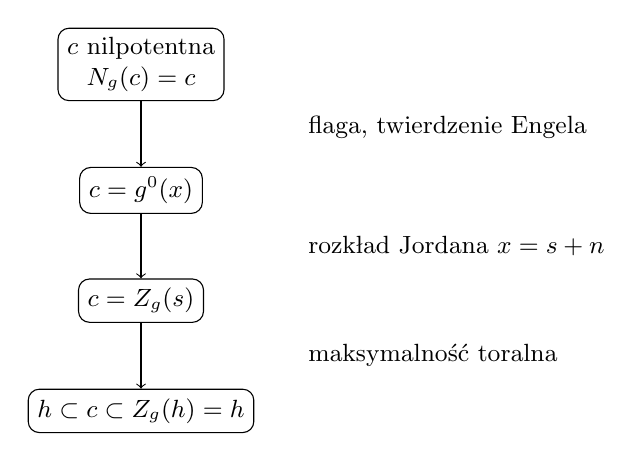
\begin{tikzpicture}[every node/.style={font=\small}]
\node[draw,rounded corners,align=center] (a) at (0,0) {$\mathfrak c$ nilpotentna\\$N_{\mathfrak g}(\mathfrak c)=\mathfrak c$};
\node[draw,rounded corners] (b) at (0,-1.6) {$\mathfrak c=\mathfrak g^0(x)$};
\node[draw,rounded corners] (c) at (0,-3.0) {$\mathfrak c=Z_{\mathfrak g}(s)$};
\node[draw,rounded corners] (d) at (0,-4.4) {$\mathfrak h\subset\mathfrak c\subset Z_{\mathfrak g}(\mathfrak h)=\mathfrak h$};
\draw[->] (a)--(b);
\draw[->] (b)--(c);
\draw[->] (c)--(d);
\node[anchor=west] at (2,-.8) {flaga, twierdzenie Engela};
\node[anchor=west] at (2,-2.3) {rozkład Jordana $x=s+n$};
\node[anchor=west] at (2,-3.7) {maksymalność toralna};
\end{tikzpicture}

\small Schemat dowodu implikacji od podalgebry Cartana do maksymalnej podalgebry toralnej.
\end{center}

\section{Przykłady i granice twierdzenia}

\begin{przyklad}[Jądro a przestrzeń zerowa Fittinga]
\label{aa:prz:lie-fitting-sl2}
W $\mathfrak{sl}_2(K)$, dla $K$ algebraicznie domkniętego charakterystyki zero, przyjmijmy $e=E_{12}$, $f=E_{21}$, $h=\operatorname{diag}(1,-1)$. Mamy $[e,h]=-2e$, $[e,f]=h$ i $[e,e]=0$. Wobec tego
$\ker\operatorname{ad}_e=Ke$, $\ker(\operatorname{ad}_e)^2=Ke+Kh$ oraz $(\operatorname{ad}_e)^3=0$. Zatem $\mathfrak g^0(e)=\mathfrak g$, chociaż zwykły centralizator $Z_{\mathfrak g}(e)$ ma wymiar jeden. Linia $Ke$ jest abelowa, lecz nie jest podalgebrą Cartana: jej normalizator to $Ke+Kh$. Istotnie, dla $y=ae+bf+ch$ mamy $[y,e]=-bh+2ce$, co należy do $Ke$ dokładnie dla $b=0$.

Dla $x=h$ sytuacja jest inna: $\operatorname{ad}_h$ ma wartości własne $2,-2,0$ na bazie $(e,f,h)$. Stąd $\mathfrak g^0(h)=Z_{\mathfrak g}(h)=Kh$, a $Kh$ jest podalgebrą Cartana na mocy Twierdzenia~\ref{aa:tw:cartan-toral-equivalence}.
\end{przyklad}

\begin{przyklad}[Konieczność półprostoty]
\label{aa:prz:cartan-nontoral}
Niech $\mathfrak n$ będzie trójwymiarową algebrą Heisenberga nad algebraicznie domkniętym ciałem charakterystyki zero, o bazie $p,q,z$ i relacjach $[p,q]=z$, $[p,z]=[q,z]=0$. Jest nilpotentna klasy dwa, a $N_{\mathfrak n}(\mathfrak n)=\mathfrak n$, więc cała $\mathfrak n$ jest podalgebrą Cartana samej siebie. Nie jest toralna, ponieważ nie jest abelowa.

Co więcej, każdy $\operatorname{ad}_x$ jest nilpotentny. Jeśli jest diagonalizowalny, musi być zerowy, czyli $x$ należy do centrum $Kz$. Maksymalną podalgebrą toralną jest zatem $Kz$, której normalizator jest równy całej $\mathfrak n$. Przykład pokazuje, że bez półprostoty obie implikacje Twierdzenia~\ref{aa:tw:cartan-toral-equivalence} mogą zawodzić.
\end{przyklad}

\begin{uwaga}
W AA-63 regularność w podalgebrze toralnej oznaczała niezerowanie wszystkich korzeni. W półprostej algebrze dla $t$ należącego do podalgebry toralnej operator $\operatorname{ad}_t$ jest diagonalizowalny, zatem $\mathfrak g^0(t)=\ker\operatorname{ad}_t$. Dla dowolnego elementu algebry nie należy bez dodatkowego argumentu utożsamiać tych przestrzeni, jak pokazuje Przykład~\ref{aa:prz:lie-fitting-sl2}.
\end{uwaga}
